\documentclass{scrartcl}

\usepackage[hidelinks]{hyperref}
\usepackage[none]{hyphenat}
\usepackage{setspace}
%\doublespace Plz no, I need to proofread this

\usepackage{graphicx}
\usepackage{float}
\graphicspath{{images/}}

\title{What C++ architecture could best support QoE-oriented map streaming in a player-building-based multiplayer game?}
\subtitle{COMP130 - Computing Architecture}
\date{\today}
\author{1707981}

\begin{document}
\maketitle
\pagenumbering{arabic}

\begin{abstract}
Low broadband speeds in large gaming markets such as China and Brazil could hinder the advancement of multiplayer gaming, particularly for traffic-hungry projects such as MMOs or building games. From a creative standpoint, player experience is decidedly the most important factor in a game's design. Low broadband bandwidth increases download speeds and strips players of valuable gaming time, causing frustration. To aid this, Quality-of-Experience (QoE) techniques are proposed to mitigate the negative effects of limited bandwidth on the player experience, in a way that could be adapted to existing games with minimal difficulty.
\end{abstract}

\section{Introduction}
\begin{figure}
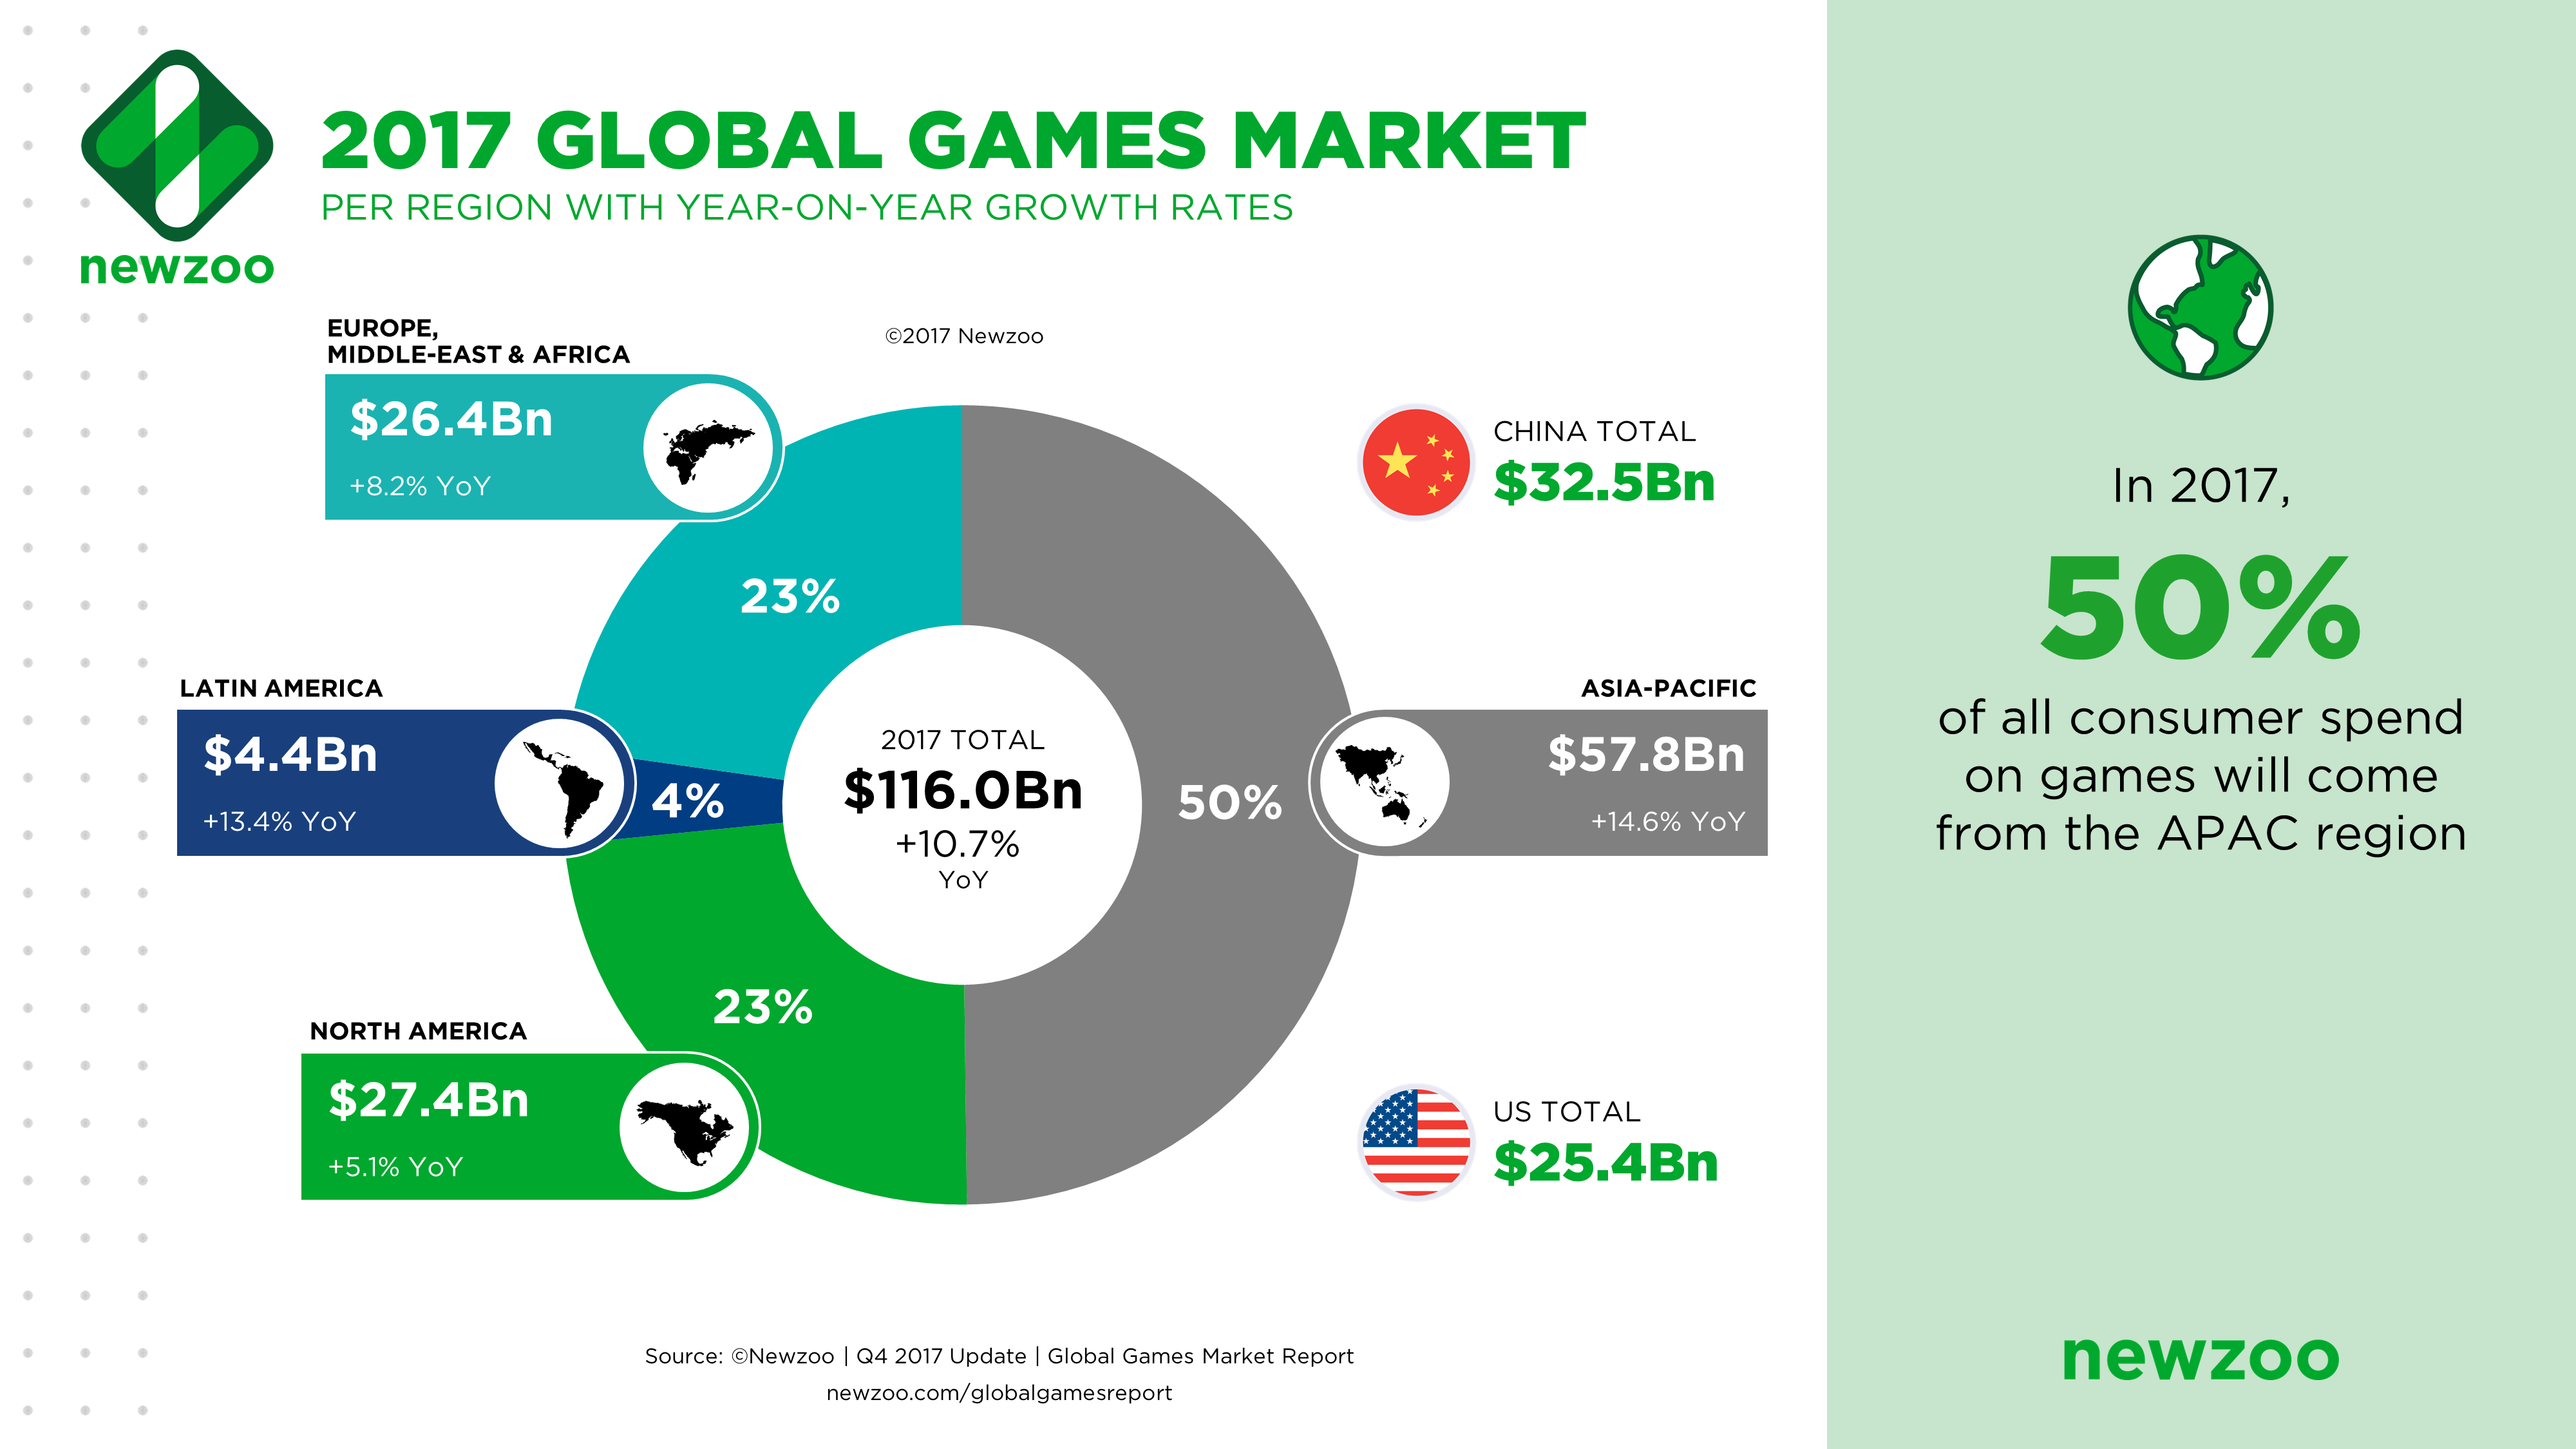
\includegraphics[width=0.75\linewidth]{Newzoo_2017_Global_Games_Market.png}
\caption{The games market in 2017, according to NewZoo}
\label{fig:market}
\end{figure}
The games market is continuing to grow at an immense rate, especially in developing countries. In East Asia, a growth of nearly 15\% over the last year has been observed.\cite{fig:market}

This presents exciting creative opportunities for game developers to expand into new territories. However, a lag in technological advancement, particularly broadband, raises reasonable concerns of whether they can fully exploit these opportunities. The potential of games where players can build the map, such as the extremely popular (as suggested by Google Trends\cite{minecraftnite}) Minecraft and Fortnite, may be hindered by a lack of bandwidth necessary to download player-built resources at an acceptable speed. This may frustrate players by rendering them unable to access areas of the game in a timely manner.

This study aims to discover the extent of this problem, followed by proposals of architectural methods to implement systems that could mitigate the negative effects on the player experience in an unreliable networking environment: This largely comprises of QoE (quality-of-experience) improvements. The programming language in question is C++, while the hypothetical game assumed a 3D environment wherein the player can manipulate the terrain and build meshes. The goal is to propose a reasonable set of design patterns to be used for QoE-oriented map streaming in a large-scale game, and how they could be applied to an existing game engine.

This analysis will take place over the following steps:
\begin{itemize}
\item Exploration into the games market, and its broadband speeds
\item A brief introduction of player experience as a separate concept to content quality
\item Existing strategies used by games for a) map streaming and b) online synchronisation, and
\item A proposed technical outline of a system that could facilitate appropriate level streaming considering the aforementioned variables.
\end{itemize}

\section{The wider market}
China is in fact the most profitable games market as of 2017 \cite{chinamarket}. Furthermore, in March 2018, 8 of the 10 most popular Steam games in China were partly or fully multiplayer \cite{steamchina}. This suggests China is a valuable target for online games, yet its Internet speeds lag behind (figuratively speaking) the world, at an average of 7.6Mbps \cite{webspeeds}.

Another country notorious for its online gaming community is Brazil, whose Internet speeds averaged about the same--6.8Mbps--in 2017.\cite{webspeeds}. While a marked improvement is evident (doubling since 2015 \cite{webspeeds2015}), to the extent that low-bandwidth games such as FPSes are comfortably playable [cite?], this low speed closes doors to potential large-scale player-built online games.

(Internet speeds in Brazil are notoriously low--an unfortunate feat for the fifth top source of DDoS attacks in early 2017\cite{websecurity}--)

\section{Player experience}
Video streaming is a heavily researched area; perhaps more than games, owing to greater dedicated R\&D toward streaming services such as the Amazon FireTV[cite?]. Considering the aesthetic link between video quality and quality of gameplay--including pixel resolution, lag spike rate, and frame rate--we can draw some preliminary conclusions about a player's interests from studies.

It has been documented \cite{qoelargestudy} that user enjoyment is greater in a scenario of low-detail, constant frame streaming, than one of higher-detail, inconsistent frame streaming. In other words, the user is not interested in the rate of high-detailed data--they are interested in enjoying a smoother experience.

A smooth experience is necessary to retain game players. Studies have noted latency \cite{qossensitivity} \cite{lagragequits}, jitter and packet loss \cite{lagragequits} to all have negative impacts, sometimes leading to quitting altogether. While this is not widely studied in building games--but FPSes and MMOs--games such as the hugely popular (cite?) Fortnite, which features building elements with shooting gameplay, suggest that there may be a demand for player building in those contexts regardless. The potential loss of players therefore justifies the development of strategies to improve the player experience on an unreliable network, especially considering the high traffic potential of level streaming.

\section{Existing strategies}
Granted, it is fair to say player experience-driven streaming already exists, though this assumes a higher data rate, and takes the form of open-world streaming from disc. Engines such as the Unreal engine provide World Composition, allowing the world to be partly loaded in small sections as the player approaches them \cite{unrealcomposition}. This is characterised by the loading of reduced LOD (Level-of-Detail) versions of areas distant to the camera, and the high LOD versions of close areas. This hides detail in the distance at the benefit of reducing the memory footprint and rendering times: both a potential improvement to the asset download time and frame rate, and consequently an improvement to the player's perception of the game.

This streaming method provides data to the player in a spatially-aware manner such that the player has fastest access to the area immediately around them. However, the key difference in the online equivalent system is the data rate. In the PS4 and Xbox One's case, static map streaming from the disc this defaults at 27MB/s (Cite this)--a significantly higher rate than China's average Internet speed of 7.6Mbps, or 0.95 MB/s. At only 4\% of the typical disc data rate, it is reasonable to question whether game level streaming is prepared for such a bottleneck.

\section{Proposal}
Due to an extreme lack of time and an extremely tired caffeine-free (and vitamin-deficient) author, a tacked-together solution is hastily proposed by this essay draft.

\begin{figure}
	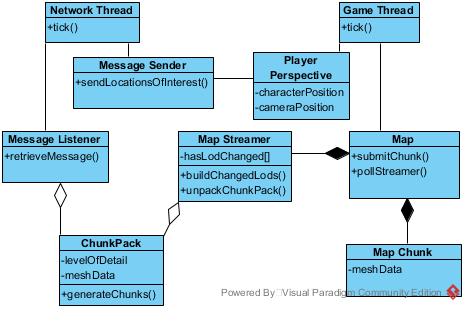
\includegraphics[width=0.7\linewidth]{Basic_Map_Streamer}
	\caption{A class diagram demonstrating a map streaming component connected to a basic Map class.}
	\label{fig:simplesystem}
\end{figure}

The class diagram above depicts the client end of the map streaming game component. As some partly-downloaded data is not needed by the game component until it's complete, the process is divided into two concurrent, non-conflicting threads. Flow takes place in the following fashion:

\begin{figure}[H]
	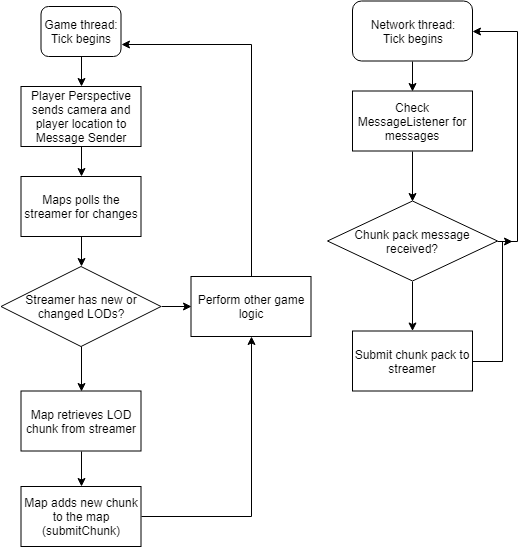
\includegraphics[width=0.7\linewidth]{Basic_Flowchart.png}
	\caption{Process flow of the two threads in parallel}
	\label{fig:simpleflow}
\end{figure}

In this example, the client begins by sending the player and camera location as soon as possible. Sometimes these two variables may be different: it is important that both areas are prepared for the player's viewing. The server is assumed to prioritise the level chunk geometry from closest to furthest.

A \textbf{level chunk} is defined as a region of space where static level geometry resides. The shape of a level chunk varies across games, though in a building game, a uniform shape could be chosen such that there are no notable inefficiencies to building in one place over another. Existing games use various strategies. For example, Sunset Overdrive (Insomniac Games, 2014) used hexagonal chunks by design and radial chunks in practice. This was optimised for the player's freedom of movement. However, an earlier game by the same company, Fuse (Insomniac Games, 2013), used rectangular chunks. This was optimised for linear hall-based gameplay. (CITE ALL THIS).

The \textbf{level streamer} is responsible for collecting \textbf{Chunk Packs} (partial, LOD-specific level chunk data downloaded from the server) and transferring them to the physical \textbf{Map} when it deems appropriate. In the above example, it does so as soon as it is immediately downloaded. However, it may benefit the player experience to record the amount of processing time spent during recent frames, and responding by slowing the conversion process or postponing it. This could help preserve a high frame rate and provide a smoother experience.

\section{Total Conclusion}
There are further systems to be explored, citations to be added and slightly passive-aggressive expressions of frustration to be passive-aggressively expressed at the recent surge in workload that are beyond the scope of this essay draft, and the author's physical capabilities at 3am, let alone intellectual ones. The author as such has little idea what they are doing and submits this draft to the peer review with great hesitation and a tear in his eye.

\bibliography{references} 
\bibliographystyle{ieeetr}

\end{document}